
\chapter{Экспериментальная часть}\label{exp}
%\addcontentsline{toc}{chapter}{4 Экспериментальная часть}

Оценка качества работы алгоритмов. Экспериментальное сравнение работы различных алгоритмов нахождения среднего арифметического матрицы
(зависимость времени выполнения от размерности матриц).

\section{Технические характеристики}\label{texcharacters}

Технические характеристики устройства, на котором выполнялось тестирование:

\begin{enumerate}
    \item процессор: Intel® Core™ i3-7100U CPU @ 2.40GHz × 4; 
    \item память: 11,6 GiB;
    \item операционная система: Ubuntu 20.04.1 LTS.
\end{enumerate}

\section{Примеры работы}\label{examples}

На рисунках \ref{ris:w1}, \ref{ris:w2} показаны примеры работы.

\begin{figure}[H]
    \center{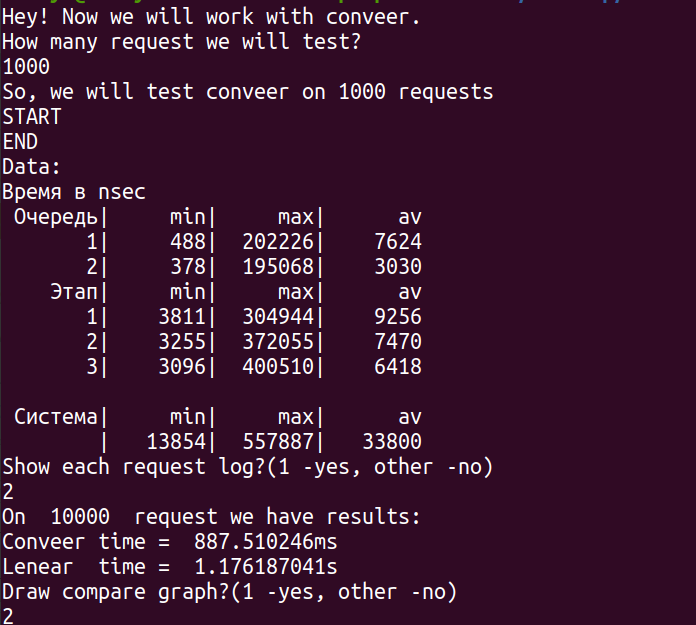
\includegraphics[scale=0.35]{w1}}
    \caption{Пример 1}
    \label{ris:w1}
\end{figure}
  
\begin{figure}[H]
    \center{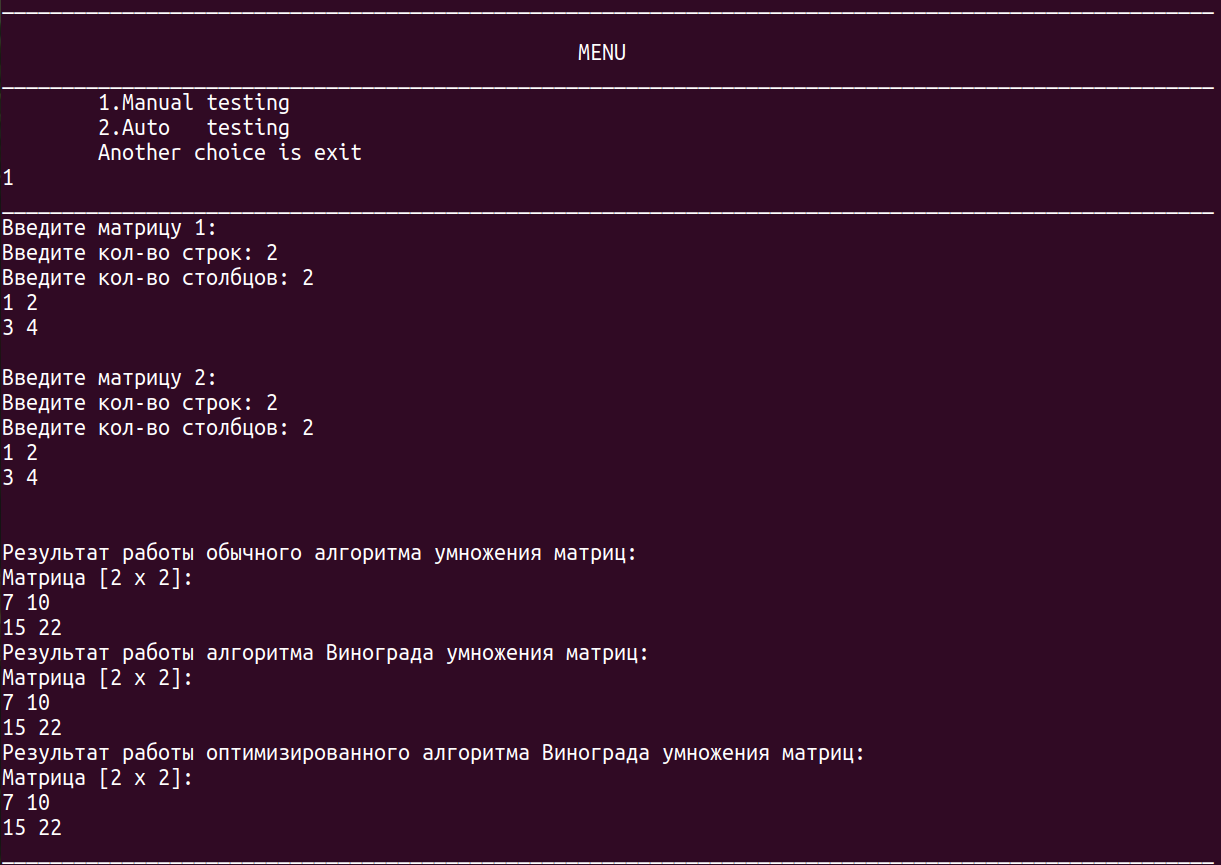
\includegraphics[scale=0.35]{w2}}
    \caption{Пример 2}
    \label{ris:w2}
\end{figure}
  
%\begin{figure}[H]
%    \center{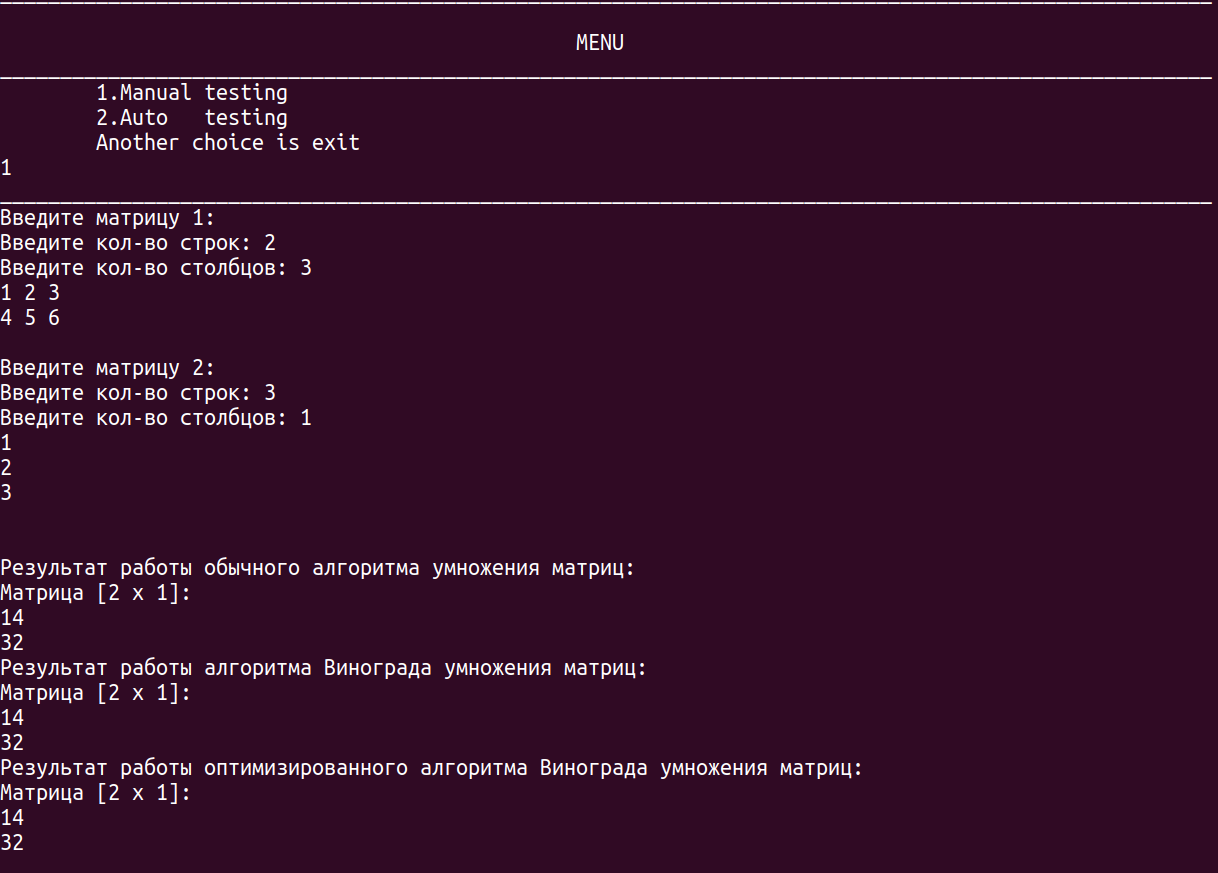
\includegraphics[scale=0.35]{w3}}
%    \caption{Ручное тестирование: тест 3}
%    \label{ris:w4}
%\end{figure}
  
%\begin{figure}[H]
%    \center{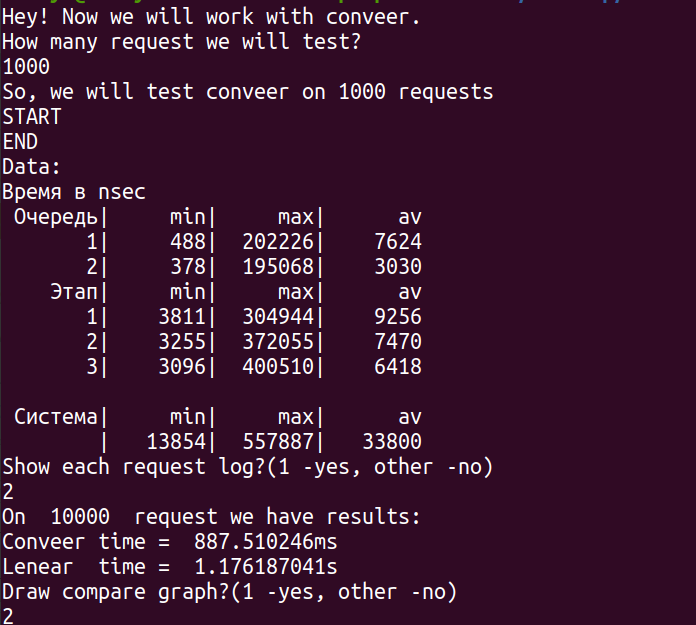
\includegraphics[scale=0.25]{w1}}
%    \caption{Автотестирование}
%    \label{ris:w3}
%\end{figure}

\section{Замеры времени}\label{experimentgraph}

Таблица \ref{tab:resulttime} содержит резульаты замеров времени при 1, 2, 4, 8, 16, 32 потоках
\begin{table}[ht]
    \caption{Замеры времени (в нсек)}
    \centering
   % \scriptsize
\begin{tabular}{ l | l | l}
    Размер матрицы&    Название алгоритма&         time\\ \hline
    2&   Полный перебор&    12.100000\\
    2&   Муравьиный алгоритм&   134.000000\\
    3&   Полный перебор&    15.200000\\
    3&   Муравьиный алгоритм&   223.800000\\
    4&   Полный перебор&    27.200000\\
    4&   Муравьиный алгоритм&   357.600000\\
    5&   Полный перебор&    74.800000\\
    5&   Муравьиный алгоритм&   755.400000\\
    6&   Полный перебор&   360.300000\\
    6&   Муравьиный алгоритм&  1132.800000\\
    7&   Полный перебор&  1433.100000\\
    7&   Муравьиный алгоритм&   501.600000\\
    8&   Полный перебор& 12348.600000\\
    8&   Муравьиный алгоритм&   668.100000\\
    9&   Полный перебор&120832.700000\\
    9&   Муравьиный алгоритм&  1051.100000\\
   10&   Полный перебор&2717589.600000\\
   10&   Муравьиный алгоритм&  7412.900000\\
\end{tabular}
\label{tab:resulttime}
\end{table}



На рисунках \ref{ris:graph1} показаны графические результаты сравнения исследуемых алгоритмов по времени. По оси X 
- размер матрицы смежности, по оси у - время выполнения в нсек.

\begin{figure}[H]
    \center{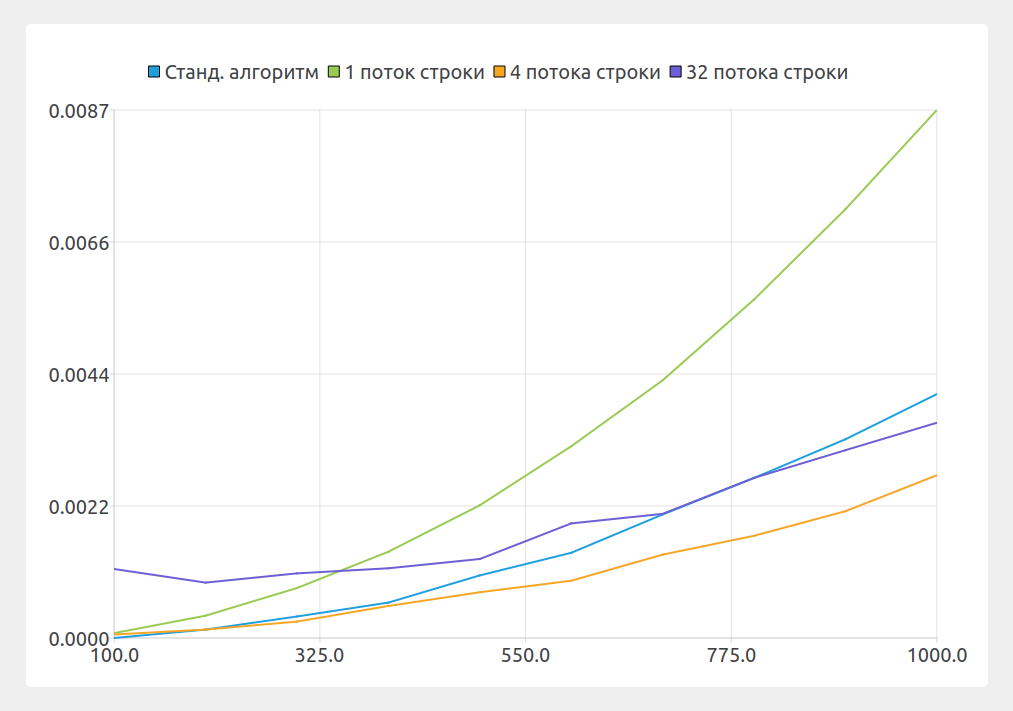
\includegraphics[scale=0.45]{graph1}}
    \caption{Сравнение алгоритма полного перебора и муравьиного алгоритма}
    \label{ris:graph2}
\end{figure}

%\begin{figure}[H]
%    \center{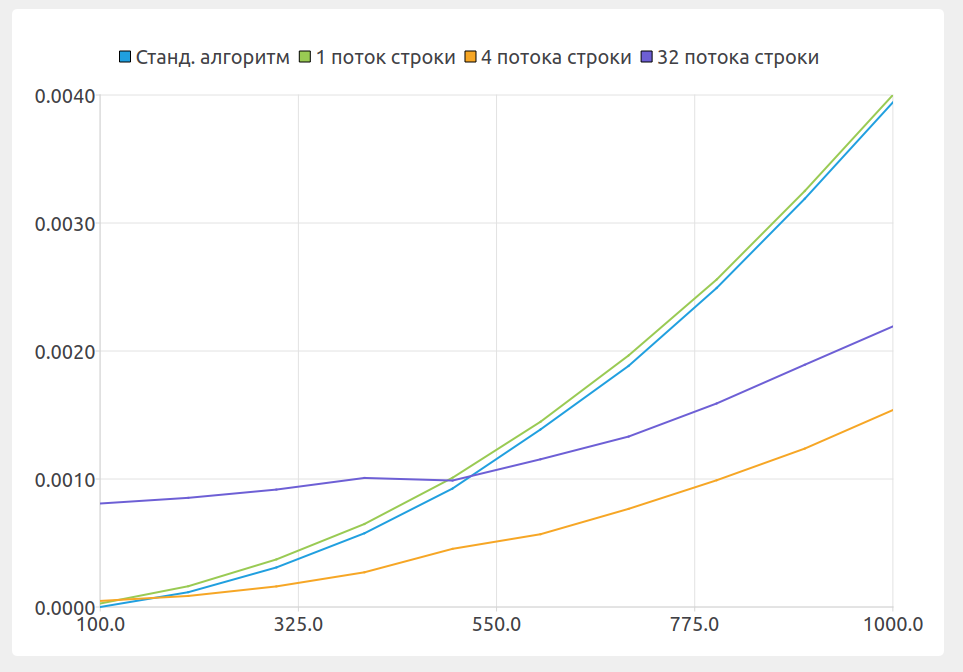
\includegraphics[scale=0.4]{graph5}}
%    \caption{Сравнение алгоритмов стандартного, распараллеленого по строкам на 1, 2, 4, 32 потока}
%    \label{ris:graph1}
%\end{figure}

\section{Параметризация муравьиного алгоритма}\label{comparepart}

В муравьином алгоритме вычисления производятся на основе настраиваемых параметров.
Рассмотрим матрицу смежностей размерностью 10 × 10.

\begin{table}[ht]
    \caption{Тестовая матрица}
    \centering
\begin{tabular}{ l | l  l  l  l  l  l  l  l  l l}
    0 & 0 & 1 & 2 & 3 & 4 & 5 & 6 & 7 & 8 & 9 \\ \hline
    0 & 0 & 1790 & 200 & 1900 & 63 & 1659 & 1820 & 1395 & 2382 & 649 \\
    1 & 1790 & 0 & 1573 & 2435 & 1515 & 714 & 892 & 2193 & 1590 & 1003 \\
    2 & 200 & 1573 & 0 & 833 & 392 & 2404 & 962 & 902 & 141 & 1123 \\
    3 & 1900 & 2435 & 833 & 0 & 2283 & 1652 & 2362 & 2262 & 1512 & 2166 \\
    4 & 63 & 1515 & 392 & 2283 & 0 & 1322 & 290 & 1305 & 2100 & 969 \\
    5 & 1659 & 714 & 2404 & 1652 & 1322 & 0 & 256 & 78 & 2236 & 2041 \\ 
    6 & 1820 & 892 & 962 & 2362 & 290 & 256 & 0 & 1180 & 1547 & 1279 \\ 
    7 & 1395 & 2193 & 902 & 2262 & 1305 & 78 & 1180 & 0 & 1640 & 1161 \\
    8 & 2382 & 1590 & 141 & 1512 & 2100 & 2236 & 1547 & 1640 & 0 & 2212 \\
    9 & 649 & 1003 & 1123 & 2166 & 969 & 2041 & 1279 & 1161 & 2212 & 0 \\
\end{tabular}
\label{tab:test_matrix}
\end{table}


Результаты тестирования представлены в таблице \ref{tab:some_res}

Параметризация метода решения задачи коммивояжера на основании
муравьиного алгоритма проводилась для матрицы с элементами в диапозоне
[0, 2500]. Количество дней было равно 50. Полный перебор определил оптимальную длину пути 6986. 
Столбец ”результат” отвечает за результат работы
муравьиного алгоритма. Столбец ”разница” отвечает за разницу с оптимальной длиной.

\begin{table}[ht]
    \caption{Тестовая матрица}
    \centering
\begin{tabular}{ l | l  | l |  l  | l}
    alpha&         beta&            p&    Результат&      Разница \\ \hline
    0.0&          1.0&          0.7&       6986.0&          0.0\\
    0.0&          1.0&          0.8&       6986.0&          0.0\\
    0.0&          1.0&          0.9&       6986.0&          0.0\\
    0.0&          1.0&          1.0&       6986.0&          0.0\\
    0.5&          0.5&          0.7&       7139.0&        153.0\\
    0.5&          0.5&          0.8&       7479.0&        493.0\\
    0.5&          0.5&          0.9&       7139.0&        153.0\\
    0.5&          0.5&          1.0&       6986.0&          0.0\\
    1.0&          0.0&          0.5&       8277.0&       1291.0\\
    1.0&          0.0&          0.6&       7329.0&        343.0\\
    1.0&          0.0&          0.7&       8185.0&       1199.0\\
    1.0&          0.0&          0.8&       6986.0&          0.0\\
\end{tabular}
\label{tab:some_res}
\end{table}


\newpage



\section{Вывод экспериментальной части}\label{experimentresult}

На основе проведенной параметризации (таблицы \ref{tab:some_res}, \ref{label}) для матрицы
смежности приведенной в таблице \ref{tab:test_matrix} рекомендуется использовать
($\alpha$ < $\beta$, $\rho$ = любое). При параметрах $\alpha = 0$,  $\beta = 1$, количество правильно
найденных оптимальных путей составило 8 единиц. При $\alpha = 0$, $\beta = 1$ 8 из 10 найденных путей были 
оптимальные.

\addcontentsline{toc}{chapter}{{Заключение}}
\chapter*{Заключение}\label{exit}

В данной лабораторной работе были рассмотрены основополагающие
материалы которые в дальнейшем потребовались при реализации алгоритма
полного перебора и муравьиного алгоритма. Были рассмотрены схемы для
решения задачи коммивояжера. Также были разобраны листинги , показывающие работу,
описанных выше алгоритмов. Был произведен сравнительный
анализ. Выполнены поставленные задачи.

